%%%%%%%%%%%%%%%%%%%%%%%%%%%%%%%%%%%%%
% Document properties and packages
%%%%%%%%%%%%%%%%%%%%%%%%%%%%%%%%%%%%%
\documentclass[a4paper,12pt,final]{memoir}
\usepackage{float}
% misc
\renewcommand{\familydefault}{bch}	% font
\pagestyle{empty}					% no pagenumbering
\setlength{\parindent}{0pt}			% no paragraph indentation
% required packages (add your own)
\usepackage{flowfram}% column layou
\usepackage{marvosym}
\usepackage{textcomp}

\usepackage[top=1cm,left=1cm,right=1cm,bottom=1cm]{geometry}% margins
\usepackage{graphicx}										% figures
\usepackage{hyperref}
\definecolor{linkcolour}{rgb}{0,0.2,0.6}  %蓝色
\hypersetup{colorlinks,breaklinks,urlcolor=linkcolour, linkcolor=linkcolour}										% URLs
\usepackage[usenames,dvipsnames]{xcolor}					% color
\usepackage{multicol}										% columns env.
	\setlength{\multicolsep}{0pt}
\usepackage{paralist}										% compact lists
\usepackage{tikz}

%%%%%%%%%%%%%%%%%%%%%%%%%%%%%%%%%%%%%
% Create column layout
%%%%%%%%%%%%%%%%%%%%%%%%%%%%%%%%%%%%%
% define length commands
\setlength{\vcolumnsep}{\baselineskip}
\setlength{\columnsep}{\vcolumnsep}
%定义主题颜色,可选颜色 Maroon,ForestGreen,DarkOrchid,RoyalBlue,Turquoise,Cyan,etc,更多颜色参考xcolor包的颜色定义
\newcommand{\myThemeColor}{RoyalBlue}
% frame setup (flowfram package)
% left frame
\newflowframe{0.23\textwidth}{\textheight}{0pt}{0pt}[left]
	\newlength{\LeftMainSep}
	\setlength{\LeftMainSep}{0.23\textwidth}
	\addtolength{\LeftMainSep}{1\columnsep}
 
% small static frame for the vertical line
\newstaticframe{1.5pt}{\textheight}{\LeftMainSep}{0pt}
 
% content of the static frame
\begin{staticcontents}{1} %绘制分割线,使用tikz包绘制。如需改变风格线样式,请参考tikz教程,对于新手,不建议修改。
\hfill
\tikz{%
	\draw[loosely dotted,color=\myThemeColor,line width=1.5pt,yshift=0]
	(0,0) -- (0,\textheight);}%
\hfill\mbox{}
\end{staticcontents}
 
% right frame
\addtolength{\LeftMainSep}{1.5pt}
\addtolength{\LeftMainSep}{1\columnsep}
\newflowframe{0.7\textwidth}{\textheight}{\LeftMainSep}{0pt}[main01]


%%%%%%%%%%%%%%%%%%%%%%%%%%%%%%%%%%%%%
% define macros (for convience)
%%%%%%%%%%%%%%%%%%%%%%%%%%%%%%%%%%%%%
\newcommand{\Sep}{\vspace{1em}}
\newcommand{\SmallSep}{\vspace{0.9em}}

\newenvironment{AboutMe}
	{\ignorespaces\textbf{\color{\myThemeColor} About me}}
	{\Sep\ignorespacesafterend}
%定义section	
\newcommand{\CVSection}[1]
	{\Large\textbf{#1}\par
	\vspace{0.2cm}\normalsize\normalfont}

\newcommand{\CVItem}[1]
	{\textbf{\color{\myThemeColor} #1}}


%%%%%%%%%%%%%%%%%%%%%%%%%%%%%%%%%%%%%
% Begin document
%%%%%%%%%%%%%%%%%%%%%%%%%%%%%%%%%%%%%
\begin{document}

% Left frame 左边内容在此定义
%%%%%%%%%%%%%%%%%%%%
\begin{figure}
	\hfill
	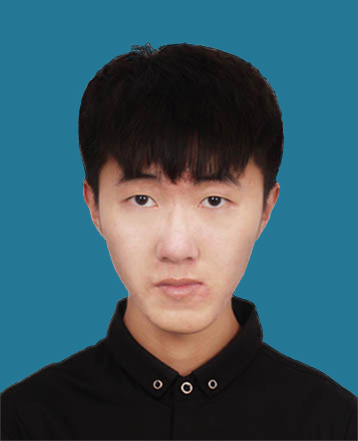
\includegraphics[width=0.8\columnwidth]{../img/photo.jpg}
	\vspace{-7cm}
\end{figure}
\begin{flushright}\footnotesize
.\\
\vskip 6cm
    \raggedright
	\CVItem{{\large Info:}}\\
	Email:\\
	\href{mailto:jiafeng5513@outlook.com}{jiafeng5513@outlook.com}  \\
	Github:\\
	\href{github.com/jiafeng5513}{github.com/jiafeng5513} \\
	Tel:\\
	15764356880
	\SmallSep
	\SmallSep

	\CVItem{{\large Skills:}}\\
	$\bullet$\textbf{Coding:}\\ C\#/C++/Java/Python\\
	$\bullet$\textbf{Major:}\\ Deep Learning/Model Deployment/HPC/Multi-Platform Client Development \\
	% \SmallSep
	% \textit{具备较丰富的桌面客户端,机器视觉和深度学习的开发经验,对U3D和UE4具有一定的使用经验,有较强的学习能力,具备英文文献查阅理解和写作能力.}

	\SmallSep
	\SmallSep
	\SmallSep
	
	\CVItem{\large Link To My Github}
	\begin{figure}[h]
		\centering
		
\includegraphics[width=0.8\columnwidth]{../img/Github.png}
	\end{figure}
	

\end{flushright}\normalsize
\framebreak


% Right frame 右边内容在此定义
%%%%%%%%%%%%%%%%%%%%
\Huge\bfseries {\color{\myThemeColor} Jia~~Feng}\\
\normalsize\normalfont

% Education
\CVSection{Time Line}
\hrule
\SmallSep

\CVItem{2022.07 - Present\hfill\textsc{Intel Asia Pacific R\&D Co., Ltd.}}\\
\textit{-Intel's Software and Advanced Technology Group (SATG)}\\
\textit{-HPC engineer}

\CVItem{2020.07 - 2022.07\hfill\textsc{Huawei Technologies Co., Ltd.}}\\
\textit{-Auto Driving Solutions BU}\\
\textit{-HPC engineer}

\CVItem{2013.09 - 2020.07\hfill\textsc{Jilin University}}\\
\textit{-School of Computer Science and Technology}\\
\textit{-Master's Degree in Computer Graphics}
\\

% CAMPU
\CVSection{Work Experience}
\hrule
\SmallSep
\CVItem{LLM Deployment\hfill\emph{Intel}}\\
\textit{$\bullet$ Supporting LLMs (DeepSeek-R1, QWen3, MiniCPM) on Intel platform, in which the Software stack is oneAPI-IPEX-torch and oneAPI-OpenVINO, Hardware is Intel x86 CPU/NPU/iGPU and Arc dGPUs. }
\\
\\
\CVItem{LLM Model and APP Development\hfill\emph{Intel}}\\
\textit{$\bullet$ 
Develop several LLM and VLM based applications on both Windows(for AIPC) and Android (for AI Cockpit), and which were exhibited at Shanghai Auto Show 2025, Import Expo 2023, and CES 2025. Work with ModelBest, develop and train GUI Agent application and model, which helps users to operate the UI of Android devices directly according to voice commands.} 
\\
\\
\CVItem{Operators Development \hfill\emph{Huawei}}\\
\textit{$\bullet$ Develop deep learning and cv operators for Huawei ADS, in which the Software stack is Mindspore and the Hardware is ARM-based Ascend610/615. The CPU operators are based on ARM SVE for some cv functions. The NPU operators are based on Huawei’s AiCore Intrinsics for the model inferences. Finished about 30 Operators in two years.}
\\
\\
\CVItem{CI/CD \hfill\emph{Huawei}}\\
\textit{$\bullet$ 
Design and develop an AI model CI/CD system for ADS Software platform, and add model conversion and operator integration processes to the CI/CD process. Enabling the entire process from training code and data source to Ascend model to be tracked by version management, which allows operator development and model conversion process to comply with Huawei ICSL specifications. }
\\
\\

% HONORS & SCHOLARSHIPS
\CVSection{Awards}
\hrule
\SmallSep
	\begin{tabular}{l|l}
		$\Rightarrow$ Intel &\textit{ Intel Employee of the Year Award in 2024.}\footnotesize\\
		$\Rightarrow$ Huawei&\textit{ Huawei Rising Star Award in 2022.}\\
		%  Won the 2024 
		%  and won the Huawei Rising Star Award.
	\end{tabular}

%%%%%%%%%%%%%%%%%%%%%%%%%%%%%%%%%%%%%
% End document
%%%%%%%%%%%%%%%%%%%%%%%%%%%%%%%%%%%%%
\end{document}